%%=============================================================================
%% Methodologie
%%=============================================================================

\chapter{\IfLanguageName{dutch}{Methodologie}{Methodology}}
\label{ch:methodologie}

%% TODO: Hoe ben je te werk gegaan? Verdeel je onderzoek in grote fasen, en
%% licht in elke fase toe welke stappen je gevolgd hebt. Verantwoord waarom je
%% op deze manier te werk gegaan bent. Je moet kunnen aantonen dat je de best
%% mogelijke manier toegepast hebt om een antwoord te vinden op de
%% onderzoeksvraag.
In dit hoofdstuk wordt besproken welke methodes er gehanteerd zijn om de resultaten te bekomen. Dit hoofdstuk is onderverdeeld in 2 delen. Ten eerste wordt er info gegeven over de 2 testomgevingen. Ten tweede wordt er besproken welke testcriteria er gekozen zijn en waarom. In deze bachelorproef wordt er vooral focus gelegd op het de praktijk, het is een praktische onderzoek.

\section{Testomgevingen}
Voor het onderzoek moeten er verschillende testomgevingen worden opgesteld, om alles in te testen. Er is een lokale virtueel  omgeving en een omgeving op cloud servers. Er is gekozen voor deze twee omgevingen omdat dit de 2 meest voorkomende omgevingen zijn in de praktijk bij server management tools. 

Ansible is al een tool die gebruikt wordt voor virtuele omgevingen door gebruikers thuis, maar ook in grote cloud omgevingen voor bedrijven. Het zou dus niet correct zijn om het alleen lokaal te testen of alleen op de cloud. 

Voor het onderzoek is dit ook interessant want er is veel meer kans op verschillende resultaten. Die kunnen dan met elkaar worden vergeleken en dan kan er worden bekeken wat de oorzaak hiervan is. Dit geeft ook een mogelijkheid om het onderzoek in de toekomst verder te onderzoeken. Waarom bijvoorbeeld Ansible beter is lokaal zonder cloud-init dan met (dit is een hypothetische stelling).

\newpage
Per omgeving is er hieronder wat meer informatie te vinden. Over het opzetten van de omgevingen zijn voor beide aparte hoofdstukken aan toegewijd, namelijk: Hoofdstuk \ref*{ch:testlokaal} en Hoofdstuk \ref*{ch:testhetzner}.

\subsection{Lokaal}
Voor de lokale omgeving zal er worden gewerkt met 2 technologieën, namelijk: VirtualBox en vagrant. 

VirtualBox is een programma waarmee je virtuele machines kunt aanmaken en beheren. Hiermee worden de servers lokaal aangemaakt. 

Het tweede programma dat wordt gebruikt is vagrant. Vagrant is een command tool die die servers configureerd. In de actieve directory wordt het commando \textit{vagrant init} gedaan, dan staat er een \textit{vagrantfile}. Dit is het bestand dat kan worden geconfigureerd naargelang de wens van de gebruiker. Daarna wordt het commando \textit{vagrant up} gedaan. Dit start de server op. De server wordt opgestart met behulp van een tool die virtuele machines beheert en aanmaakt. In dit geval dus VirtualBox.
\begin{figure}[!htb]
	\center{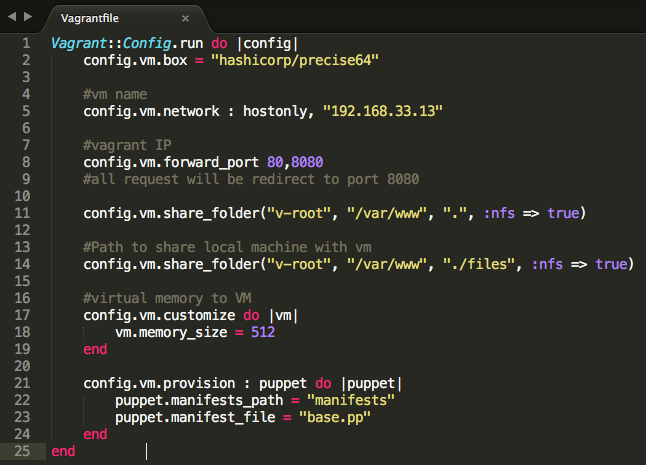
\includegraphics[width=0.9\textwidth]{img/vagrantexamp.png}}
	\caption{Voorbeeld van een vagrantfile.}
	\label{fig:vagrantexamp}
\end{figure}

\newpage
\subsubsection{Laptop}
Deze testomgeving wordt opgezet op de laptop: \textbf{Asus X750L}. Asus bracht deze laptop eind 2013 op de markt. De laptop is aangekocht in augustus 2014, en is bij het uitvoeren van het onderzoek bijna 5 jaar oud. Bijna alle specificaties zijn hetzelfde toen hij werd aangekocht. Alleen is de harde schijf vervangen van een HDD van 500 gigabyte naar een SSD van 500 gigabyte. Deze vervanging werd begin 2019 gedaan en bij het uit voeren van het onderzoek is dat 2-3 maand geleden. Hieronder is een  uitgebreide tabel met specificaties van de laptop. De data is verkregen door: \autocite{asuslaptop}.

\begin{table}
	\centering
	\begin{tabular}{c l}
		\hline
		\multicolumn{2}{c}{\textbf{Specificaties}} \\
		\hline
		Fabrikant & Asus \\
		\hline
		Model & ASUS x750L \\
		\hline		
        Besturingssysteem & Windows 10\\
        \hline
		CPU & Intel Core i7 4500U @ 2.4 GHz  \\
		\hline
		Geheugen & 8GB DDR3 @ 1600MHz \\
		\hline
		GPU & Nvidia GeForce GT 740M \\
		\hline
		Interne schijven & Crucial MX500 (500 GB) \\
		\hline
	\end{tabular}
	\caption{Specificaties van de laptop.}
	\label{tab:specs_desktop }
\end{table}

\begin{figure}[!htb]
	\center{
\includegraphics[width=0.4\textwidth]{img/testpcasus.jpg}}
	\caption{Foto van de laptop.}
	\label{fig:asustest}
\end{figure}

\subsection{Cloud}
Voor de cloud omgeving wordt er Hetzner Cloud gebruikt. In de inleiding is het bedrijf Be-Mobile al vernoemd en werd ook al gezegd dat zijn één van de redenen van het onderzoek zijn. Via hun is er toegang verkregen op een Hetzner Cloud omgeving om in te testen. 

Hetzner is een Duits bedrijf dat gespecialiseerd is in het hosten van servers. Hun datacenters liggen in Nuremberg (Duitsland), Falksenstein (Duitsland) en Helsinki (Finland). 

Via de commandline tool werden de server aangemaakt. Ook wordt er een SSH sleutel voorzien zodat er toegang is tot de aangemaakte servers. Info van hetzner werd gevonden dankzij de site van \autocite{hetzner}.


\section{Testcriteria}
Het volgende dat wordt besproken is de keuze van de testcriteria die werd gekozen in hoofdstukken~\ref{ch:basisconf},~\ref{ch:serverconf},~\ref{ch:naopstarten} en~\ref{ch:container}. 

In Hoofdstuk \ref*{ch:basisconf} worden basis configuraties op de server uit gevoerd. Dit om te bekijken wat de beste optie is om te kiezen als er gewoon wat kleine basis configuraties worden veranderd. Dit kan gebruikers aanmaken zijn, maar ook: commando's uitvoeren, mappen aanmaken. 

In Hoofdstuk \ref*{ch:serverconf} worden verschillende servers geïnstalleerd. Zo wordt er bekeken of het installeren en configureren van servers een ander resultaat heeft dan basis configuraties. Ook om te bekijken of er verschillen zijn per server.

In Hoofdstuk \ref*{ch:naopstarten} gaat er worden gekeken met welke optie je de server best aanpast na het opstarten. Als de server al opgestart is maar er wordt een klein dingetje verandert in het script. Welke optie is dan het best om snel deze verandering door te voeren.

Ten laatste wordt er in Hoofdstuk \ref*{ch:container} gekeken naar de configuratie van containers en clusters. Bijna elk bedrijf gebruikt containers en clusters voor hun netwerk. Het is dus logisch om te bekijken wat hier de resultaten zijn. Misschien zijn deze wel helemaal anders dan de resultaten van hiervoor.

\glossary{test}
%% Basis Configuratie, sever inst en conf, instellingen aanpassen na opstarten en container/cluster.

